% Waves and Oscillations
% Demonstrates: standing waves, superposition, damped oscillations, and wave packets.
% Compile with: pdflatex main.tex

\documentclass{article}
\usepackage{pgfplots}
\pgfplotsset{compat=1.18}
\usepackage{amsmath}

\title{Waves and Oscillations}
\author{LaTeX Tutorial}
\date{\today}

\begin{document}
\maketitle

% =============================================================================
\section{Traveling Wave}
% =============================================================================

A sinusoidal wave $y(x) = A\sin(kx)$:

\begin{center}
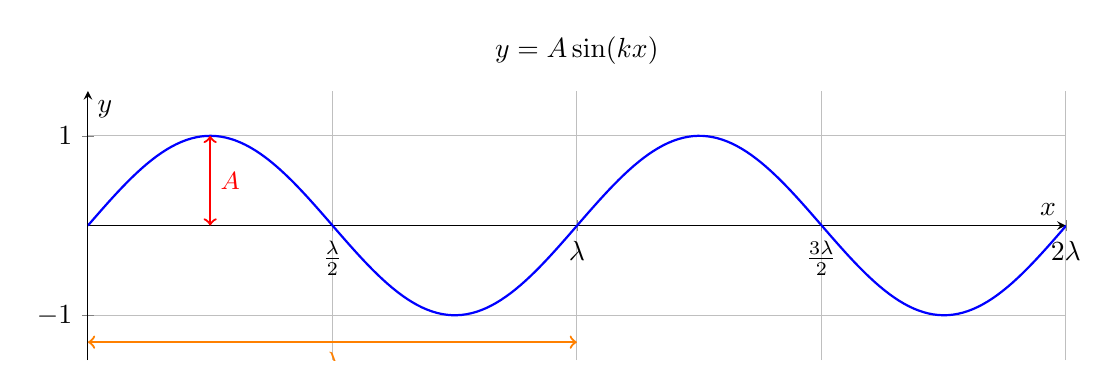
\begin{tikzpicture}
\begin{axis}[
    width=14cm, height=5cm,
    title={$y = A\sin(kx)$},
    xlabel={$x$}, ylabel={$y$},
    xmin=0, xmax=12.56, ymin=-1.5, ymax=1.5,
    grid=major,
    xtick={0, 3.14, 6.28, 9.42, 12.56},
    xticklabels={$0$, $\frac{\lambda}{2}$, $\lambda$, $\frac{3\lambda}{2}$, $2\lambda$},
    axis lines=middle,
    samples=200,
]
    \addplot[thick, blue, domain=0:4*pi] {sin(deg(x))};

    % Amplitude annotation
    \draw[<->, thick, red] (axis cs:1.57, 0) -- (axis cs:1.57, 1)
        node[midway, right, font=\small] {$A$};

    % Wavelength annotation
    \draw[<->, thick, orange] (axis cs:0, -1.3) -- (axis cs:6.28, -1.3)
        node[midway, below, font=\small] {$\lambda$};
\end{axis}
\end{tikzpicture}
\end{center}

% =============================================================================
\section{Standing Wave (Harmonics)}
% =============================================================================

First three harmonics of a string fixed at both ends:

\begin{center}
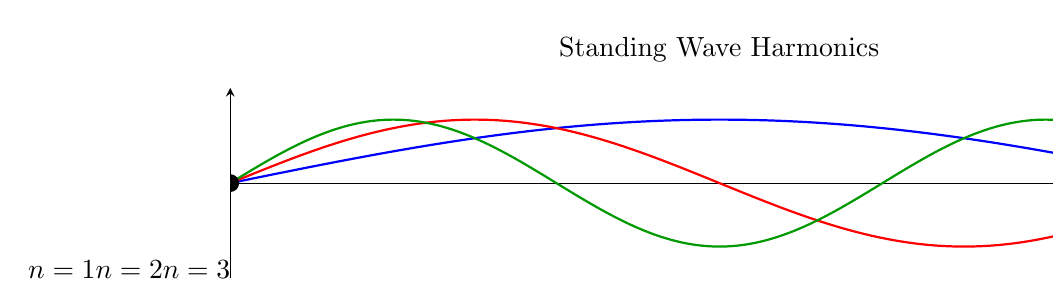
\begin{tikzpicture}
\begin{axis}[
    width=14cm, height=4cm,
    title={Standing Wave Harmonics},
    xlabel={Position $x$},
    xmin=0, xmax=3.14,
    ymin=-1.5, ymax=1.5,
    xtick={0, 3.14},
    xticklabels={$0$, $L$},
    ytick=\empty,
    axis lines=middle,
    samples=200,
    legend pos=outer north east,
]
    % n=1 (fundamental)
    \addplot[thick, blue, domain=0:pi] {sin(deg(x))};
    \addlegend{$n=1$}

    % n=2 (first overtone)
    \addplot[thick, red, domain=0:pi] {sin(deg(2*x))};
    \addlegend{$n=2$}

    % n=3 (second overtone)
    \addplot[thick, green!60!black, domain=0:pi] {sin(deg(3*x))};
    \addlegend{$n=3$}

    % Fixed endpoints
    \filldraw (axis cs:0,0) circle (3pt);
    \filldraw (axis cs:3.14,0) circle (3pt);
\end{axis}
\end{tikzpicture}
\end{center}

% =============================================================================
\section{Interference: Superposition}
% =============================================================================

Two waves and their sum (constructive and destructive interference):

\begin{center}
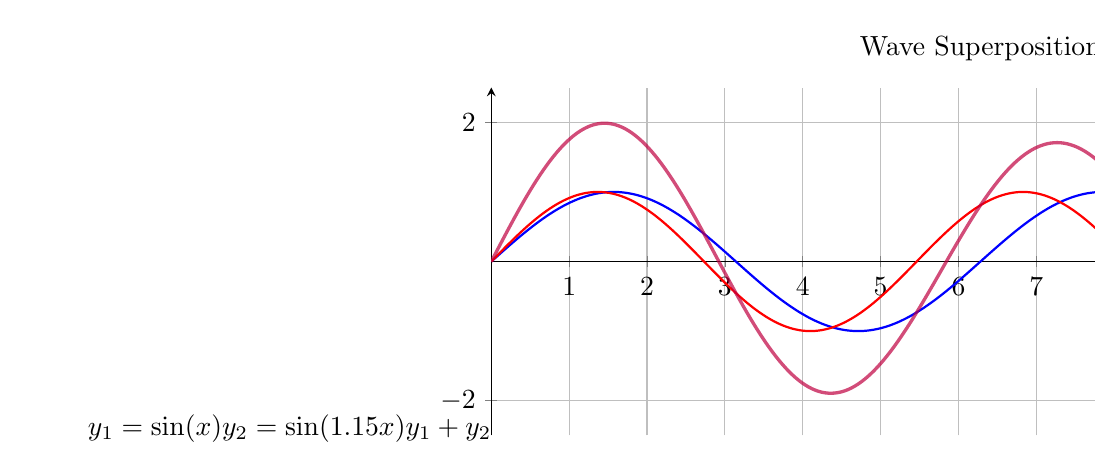
\begin{tikzpicture}
\begin{axis}[
    width=14cm, height=6cm,
    title={Wave Superposition},
    xlabel={$x$},
    xmin=0, xmax=12.56,
    ymin=-2.5, ymax=2.5,
    grid=major,
    axis lines=middle,
    samples=300,
    legend pos=outer north east,
]
    % Wave 1
    \addplot[thick, blue, domain=0:4*pi] {sin(deg(x))};
    \addlegend{$y_1 = \sin(x)$}

    % Wave 2 (slightly different frequency)
    \addplot[thick, red, domain=0:4*pi] {sin(deg(1.15*x))};
    \addlegend{$y_2 = \sin(1.15x)$}

    % Superposition (beats)
    \addplot[very thick, purple, domain=0:4*pi, opacity=0.7]
        {sin(deg(x)) + sin(deg(1.15*x))};
    \addlegend{$y_1 + y_2$ (beats)}
\end{axis}
\end{tikzpicture}
\end{center}

% =============================================================================
\section{Damped Oscillation}
% =============================================================================

$x(t) = A e^{-\gamma t}\cos(\omega t)$ for different damping levels:

\begin{center}
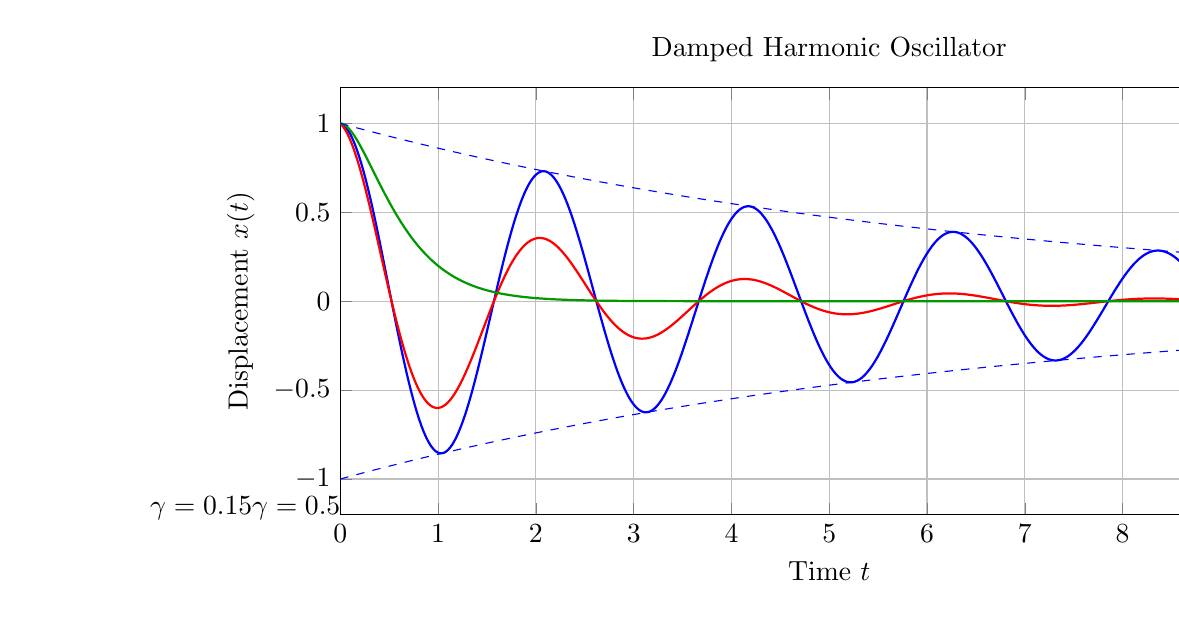
\begin{tikzpicture}
\begin{axis}[
    width=14cm, height=7cm,
    title={Damped Harmonic Oscillator},
    xlabel={Time $t$}, ylabel={Displacement $x(t)$},
    xmin=0, xmax=10,
    ymin=-1.2, ymax=1.2,
    grid=major,
    samples=400,
    legend pos=north east,
]
    % Underdamped (gamma = 0.15)
    \addplot[thick, blue, domain=0:10]
        {exp(-0.15*x) * cos(deg(3*x))};
    \addlegend{Underdamped ($\gamma=0.15$)}

    % Moderately damped (gamma = 0.5)
    \addplot[thick, red, domain=0:10]
        {exp(-0.5*x) * cos(deg(3*x))};
    \addlegend{Moderate ($\gamma=0.5$)}

    % Critically damped (gamma = 3, omega_d ≈ 0)
    \addplot[thick, green!60!black, domain=0:10]
        {(1 + 3*x) * exp(-3*x)};
    \addlegend{Critically damped}

    % Envelope for underdamped
    \addplot[dashed, blue, thin, domain=0:10] {exp(-0.15*x)};
    \addplot[dashed, blue, thin, domain=0:10] {-exp(-0.15*x)};
\end{axis}
\end{tikzpicture}
\end{center}

% =============================================================================
\section{Electromagnetic Wave}
% =============================================================================

Orthogonal $\vec{E}$ and $\vec{B}$ fields propagating along $z$:

\begin{center}
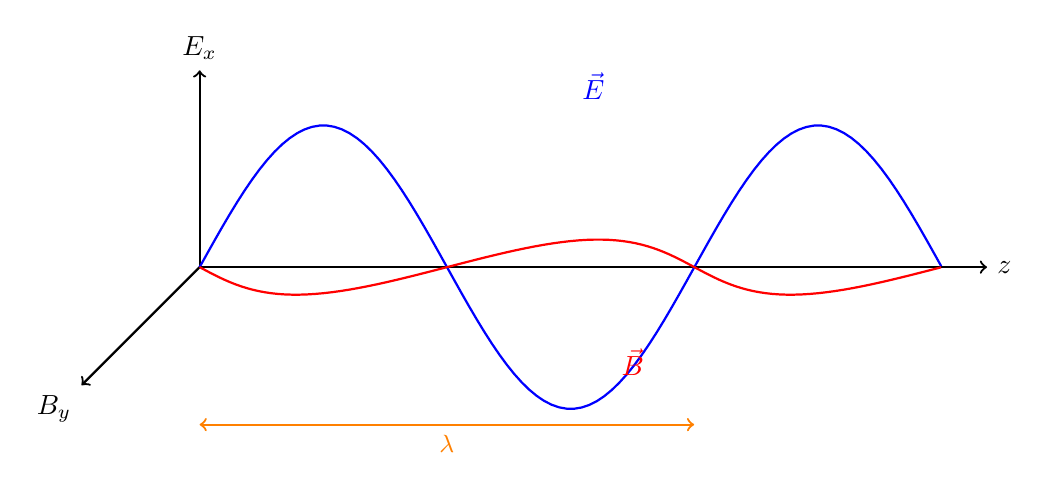
\begin{tikzpicture}
    % Propagation axis
    \draw[->, thick] (0,0) -- (10,0) node[right] {$z$};
    \draw[->, thick] (0,0) -- (0,2.5) node[above] {$E_x$};
    \draw[->, thick] (0,0) -- (-1.5,-1.5) node[below left] {$B_y$};

    % E-field (vertical sinusoid)
    \draw[thick, blue, domain=0:9.42, samples=100]
        plot (\x, {1.8*sin(deg(\x))});

    % B-field (into page / tilted sinusoid)
    \draw[thick, red, domain=0:9.42, samples=100]
        plot ({\x - 0.35*sin(deg(\x))}, {-0.35*sin(deg(\x))});

    % Labels
    \node[blue, font=\bfseries] at (5, 2.3) {$\vec{E}$};
    \node[red, font=\bfseries] at (5.5, -1.2) {$\vec{B}$};

    % Wavelength
    \draw[<->, thick, orange] (0, -2) -- (6.28, -2)
        node[midway, below, font=\small] {$\lambda$};
\end{tikzpicture}
\end{center}

\end{document}
